% This must be in the first 5 lines to tell arXiv to use pdfLaTeX, which is strongly recommended.
\pdfoutput=1
% In particular, the hyperref package requires pdfLaTeX in order to break URLs across lines.

\documentclass[11pt]{article}

% Remove the "review" option to generate the final version.
\usepackage{acl}

% Standard package includes
\usepackage{times}
\usepackage{latexsym}

% For proper rendering and hyphenation of words containing Latin characters (including in bib files)
\usepackage[T1]{fontenc}
% For Vietnamese characters
% \usepackage[T5]{fontenc}
% See https://www.latex-project.org/help/documentation/encguide.pdf for other character sets

% This assumes your files are encoded as UTF8
\usepackage[utf8]{inputenc}

% This is not strictly necessary, and may be commented out,
% but it will improve the layout of the manuscript,
% and will typically save some space.
\usepackage{microtype}

\usepackage{graphicx}
\graphicspath{ {../images/} }
\usepackage{multirow}

% If the title and author information does not fit in the area allocated, uncomment the following
%
%\setlength\titlebox{<dim>}
%
% and set <dim> to something 5cm or larger.

\title{Détermination du parti politique auquel appartient l’orateur}

% Author information can be set in various styles:
% For several authors from the same institution:
% \author{Author 1 \and ... \and Author n \\
%         Address line \\ ... \\ Address line}
% if the names do not fit well on one line use
%         Author 1 \\ {\bf Author 2} \\ ... \\ {\bf Author n} \\
% For authors from different institutions:
% \author{Author 1 \\ Address line \\  ... \\ Address line
%         \And  ... \And
%         Author n \\ Address line \\ ... \\ Address line}
% To start a seperate ``row'' of authors use \AND, as in
% \author{Author 1 \\ Address line \\  ... \\ Address line
%         \AND
%         Author 2 \\ Address line \\ ... \\ Address line \And
%         Author 3 \\ Address line \\ ... \\ Address line}

\author{Eve Sauvage \\
  Université Paris Nanterre \\
  \texttt{41017970@parisnanterre.fr}}

\begin{document}
\maketitle
\begin{abstract}
Ce document explore l'analyse d'opinion à partir d'un corpus regroupant un ensemble de débats au Parlement européen en trois langues: le français, l'anglais et l'italien. L'objectif de la tâche est d'assigner correctement les partis politiques aux interventions des parlementaires. Nous utiliserons pour cela plusieurs modèles d'apprentissage artificiel afin de déterminer un modèle idéal.
\end{abstract}

\section{Introduction}

\subparagraph{}
La tâche visée par ce document est proposée par l'édition 2009 du défi fouille de texte organisé par l'université Paris Saclay. Cette édition se concentre sur l'analyse d'opinion multilingue La tâche 3 explorée par ce document vise à l'affectation des interventions au parlement européen à des partis politiques. Les corpus utilisés pour l'entraînement et la vérification des modèles sont fournis en français, anglais et italien.
\subparagraph{}
Dans nos expériences, on suppose que la différences entre les langues nécessite que les modèles soient entraînés séparemments. Nous chercherons d'abord à déterminer le meilleur modèle sur le français avant d'essayer d'observer son efficacité sur l'anglais et l'italien. Le modèle choisi sera réentraîné sur les langues en question pour une plus grande adaptabilité.
\subparagraph{}
Cette tâche de classification a déjà été réalisée sur le corpus français par (Forest et al., 2009) avec les résultats présentés dans la Table~\ref{tab:etatArt}. Un des objectifs sera donc d'améliorer les résultats obtenus par l'équipe de Montréal en 2009.
\subparagraph{}
Une évaluation humaine de la tâche a également été réalisée. Des difficultés de classifications émergent entre les deux grands groupes politiques PSE et PPE-DE et les groupes politiques aux idéologies proches comme ELDR (centre-droit) et PPE-DE (droite) (Groin et al., 2009). Les faibles résultats de précision et de rappel obtenus par les annotateurs humains rendent bien compte de la difficulté de la tâche proposée.
\subparagraph{}
Toutefois, avec l'évolution des méthodes d'apprentissage depuis 10 ans, nous espérons observer une nette amalioration des résultats comparativement aux résultats obtenus par (Forest et al.) en 2009.

 \begin{table}[h]
 \begin{tabular}{lcccc}
 \hline
 Parti & Rappel & Précision & F-mesure\\
 \hline
 ELDR & 0,189 & 0,210 &\multirow{5}{*}{0, 320}\\
 GUE-NGL & 0,393 & 0,447\\
 PPE-DE & 0,427 & 0,447\\
 PSE & 0,360 & 0,365 \\
 Verts-ALE & 0,233 & 0,226\\
 \hline
 ELDR & 0,231 & 0,236 &\multirow{5}{*}{0, 339}\\
 GUE-NGL & 0,332 & 0,422\\
 PPE-DE & 0,498 & 0,452\\
 PSE & 0,394 & 0,370 \\
 Verts-ALE & 0,207 & 0,252\\
 \hline
  ELDR & 0,202 & 0,205 &\multirow{5}{*}{0, 334}\\
 GUE-NGL & 0,376 & 0,384\\
 PPE-DE & 0,462 & 0,462\\
 PSE & 0,383 & 0,369 \\
 Verts-ALE & 0,243 & 0,255\\
 \hline
 \end{tabular}
 \caption{Rappels et précisions obtenus par parti politique pour chacune des trois soumissions de la tâche 3 par l’équipe de Montréal.}
 \label{tab:etatArt}
 \end{table}

\section{Traitement des données}

\subparagraph{}
Les fichiers de corpus sont disponibles au format xml ce qui permet de récupérer aisement leur contenu à l'aide de la bibliothèque python \texttt{xml.etree.ElementTree} qui permet d'accéder directement aux noeuds du fichier grâce à leur nom. Les données d'entraînement sont séparées en deux listes ordonnées contenant le texte d'un côté et les étiquettes correspondantes de l'autre.
\subparagraph{}
Nous decidons d'entraîner le modèle sur la totalité des données d'entraînement et de récupérer les annotations de référence pour vérifier nos résultats. Les deux nouvelles listes obtenues sont nettoyées des résultats vides afin d'éviter les erreurs lors du décompte des résultats.
\subparagraph{}
Dans un premier temps, nous realiserons la vectorisation du texte à l'aide du TF-IDF proposé par la bibliothèque \texttt{scikit-learn} sans lemmatisation du texte d'origine. Nous réviserons cette approche au vu des résultats.
\subparagraph{}
Tous les modèles utilisés sont issus de cette même bibliothèque et adaptés au besoin de la tâche visée.

\section{Résultats}

\subsection{Arbres de décisions}

\subparagraph{}
Nous entraînons d'abord les données à l'aide d'un modèle d'arbre de décision : un modèle simple et permettant une visualisation. Ce premier modèle simple constitura notre modèle baseline avec lequel nous comparerons nos prochains essais.

\begin{table}[h]
\centering
\begin{tabular}{lcccc}
\hline
 & precision & recall & f-score\\
\hline
ELDR & 0.72 & 0.67 & 0.70 \\
GUE-NGL & 0.75 & 0.75 & 0.75\\
PPE-DE & 0.76 & 0.78 & 0.77\\ 
PSE &  0.73 & 0.73 & 0.73 \\ 
Verts-ALE & 0.69 & 0.67 & 0.68\\
\hline
accuracy& & & 0.74 \\
macro avg & 0.73 & 0.72 & 0.73\\
weighted avg & 0.74 & 0.74 & 0.74\\
\hline
\end{tabular}
\caption{rapport de classification pour le modèle arbre de décision}
\end{table}

\begin{figure}[h]
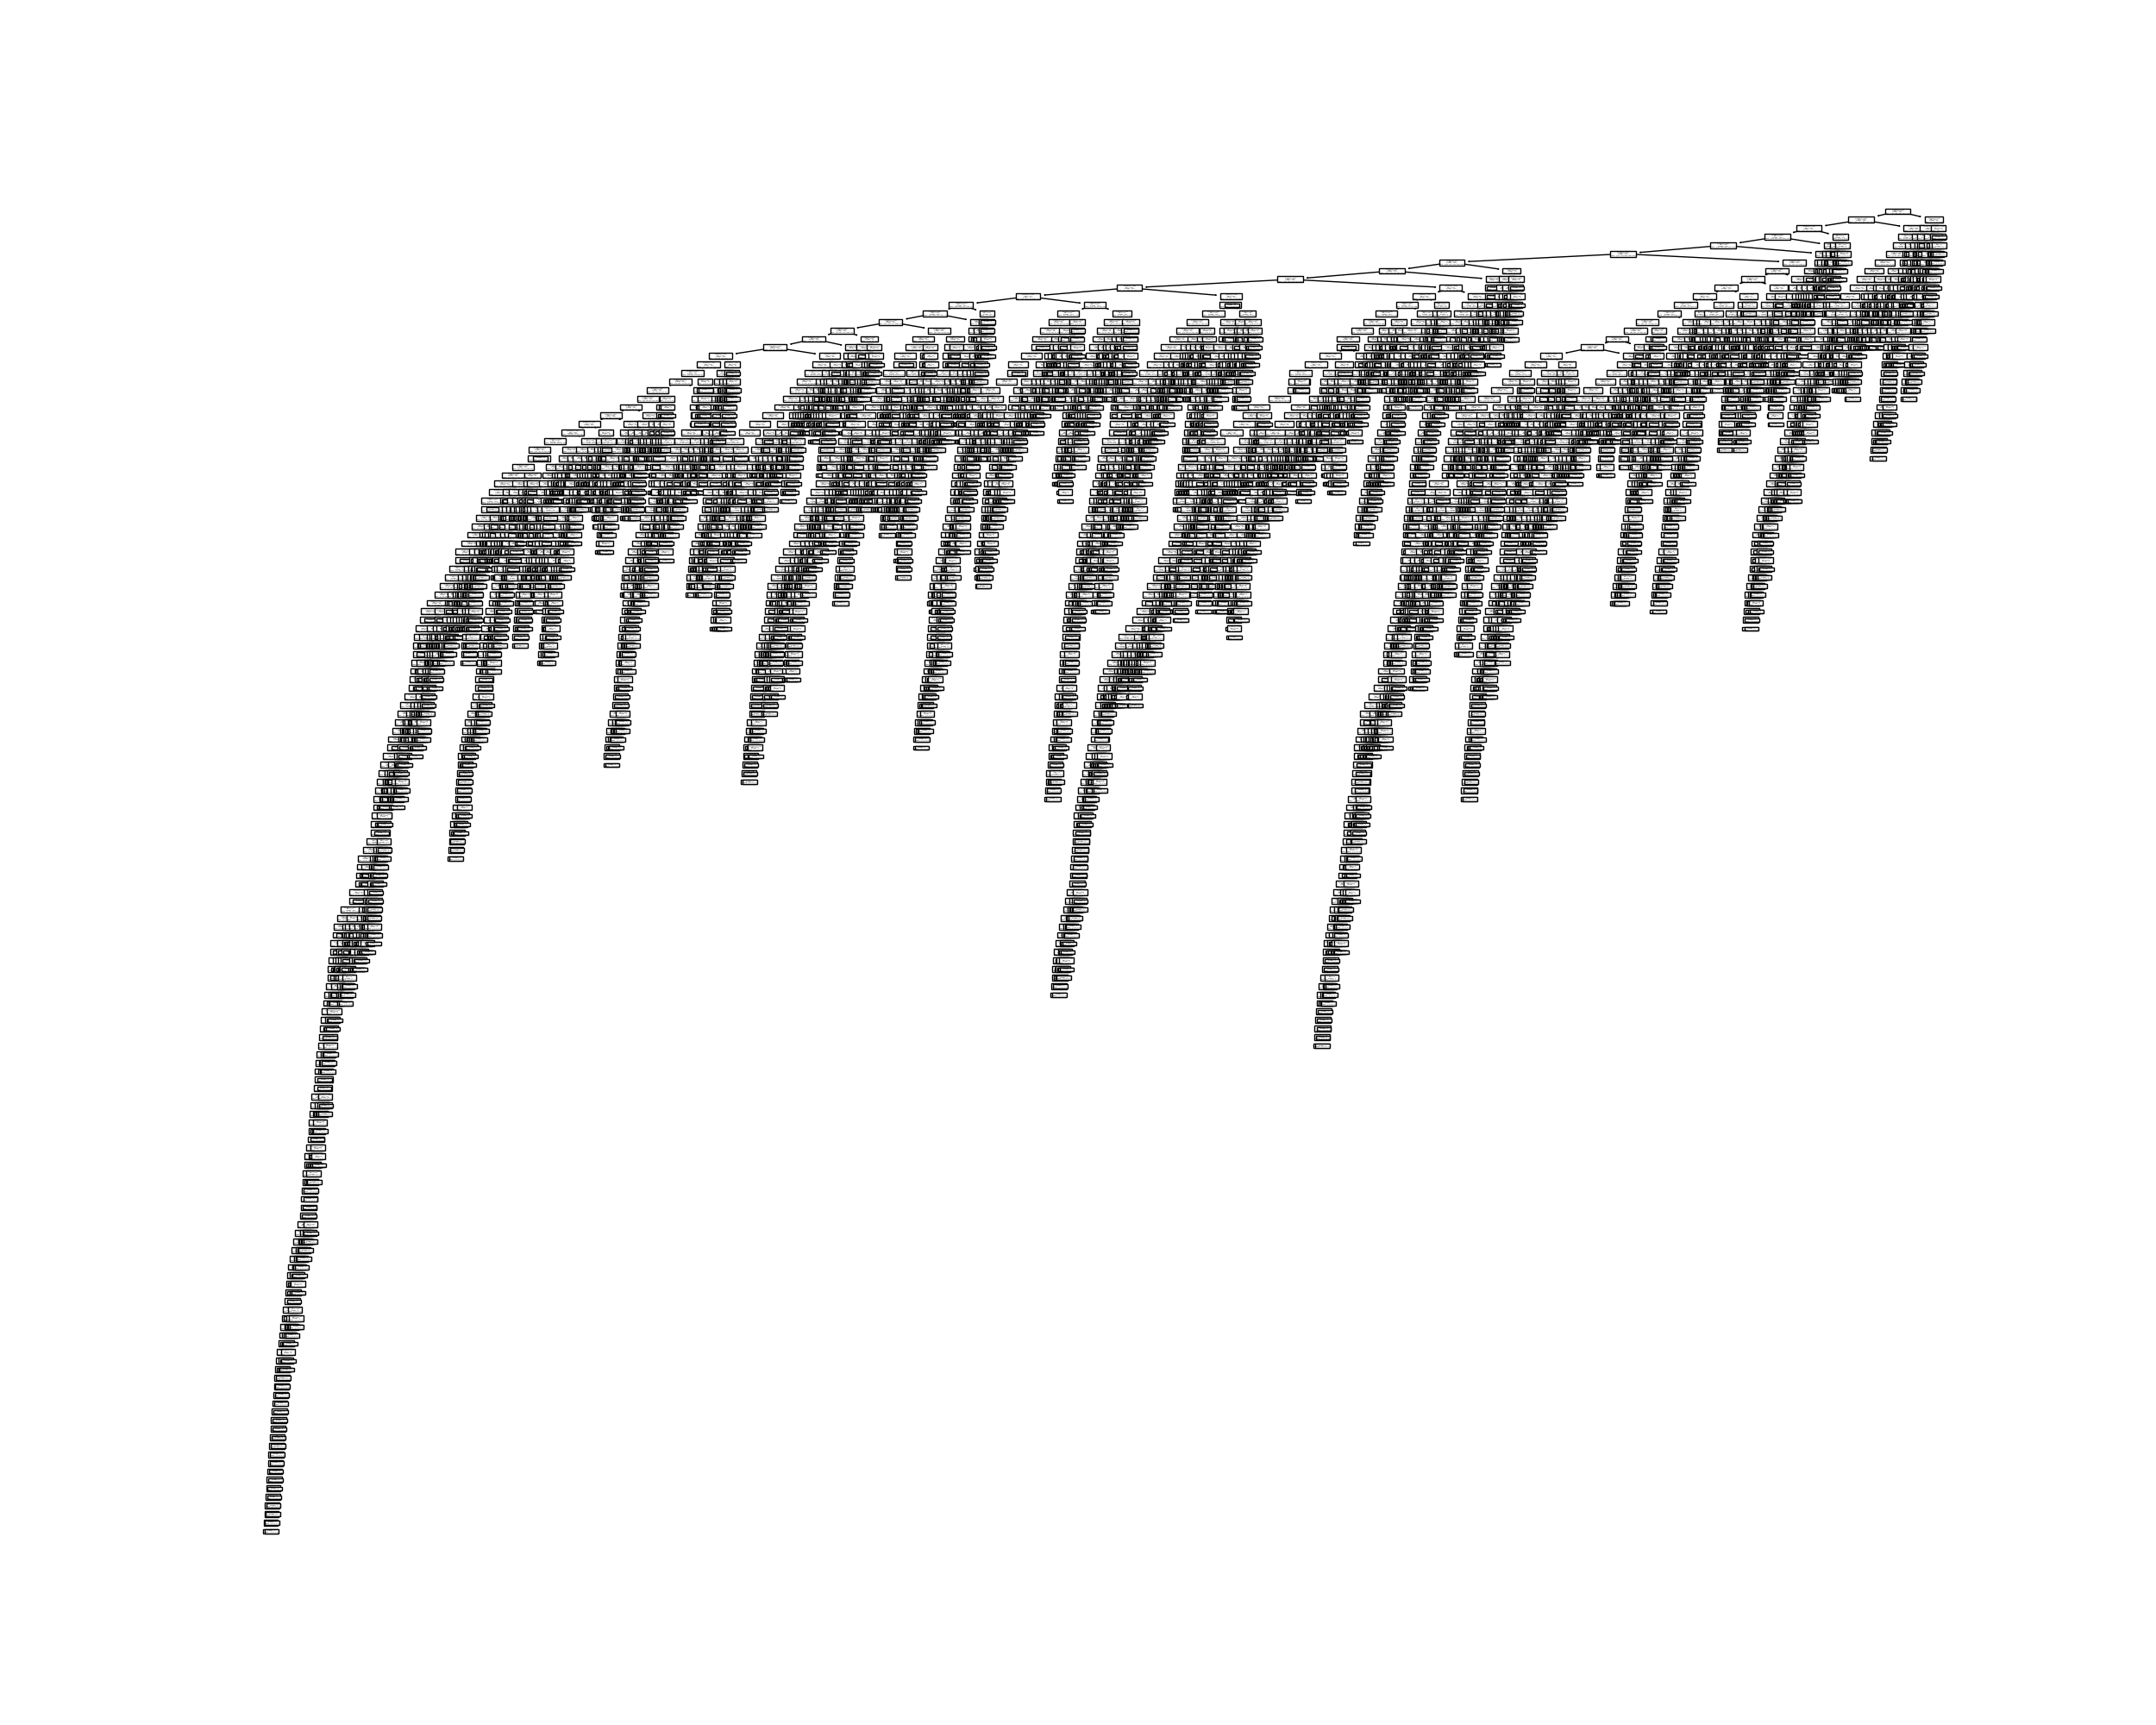
\includegraphics[width=0.5\textwidth]{decision_tree}
\caption{représentation du modèle}
\centering
\end{figure}

\begin{figure}[h]
\includegraphics[width=0.5\textwidth]{MatriceConfusionTree}
\caption{Matrice de confusion pour l'arbre de décision}
\centering
\end{figure}

\subparagraph{}
Ce premier modèle confirme notre hypthèse d'amélioration notable des résultats comparés aux soumissions de Forest et al. en 2009. Toutefois, il semble, en visualisant l'arbre de décision obtenu, que le modèle surapprend les données fournies. Ce surapprentissage est lié à l'absence de restriction de profondeur ainsi qu'à la multiplicité des paramètres entaîné par l'utilisation d'un TF-IDF pour la vectorisation des données. Il est donc pertinent de réduire le nombre de paramètres pour utiliser pleinement le potentiel de visualisation du modèle.
\subsubsection{lemmatisation et suppression des mots stops}
Nous supposons que la suppression de la ponctuation ainsi que sa lemmatisation et la suppression des mots stops amélioreront la profondeur du modèle d'arbre de décision. Toutefois, les expériences montrent que les résultats se détériorent et que la profondeur augmente. 
\subsubsection{Réequilibrage des données}
\subparagraph{}
On essaie également de réequilibrer les données d'entrainement afin de supprimer le biais du modèle mais si la précision et le rappel s'améliorent dans les classes minoritaires, les très mauvais résultats dans les classes réequilibrées, c'est à dire les classes majoritaires, nous invite à conserver le biais de départ afin de conserver une f-mesure acceptable. Les mauvais résultats dans les classes majoritaires persistent lorsque l'on rééquilibre également les données de tests. En revanche, le rééquilibrage des données permet d'effectivement diminuer la profondeur de l'arbre en utilisant un rééquilibrage par downsampling en passant d'un profondeur de 146 à une prodondeur de 96.

\begin{figure}[h]
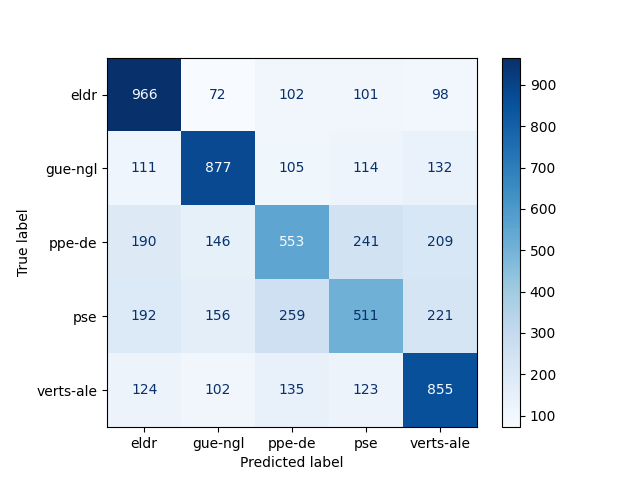
\includegraphics[width=0.5\textwidth]{matriceConfusionTreeBalanced}
\caption{Matrice de confusion avec apprentissage sur des données rééquilibrées en downsampling}
\centering
\end{figure}

\subparagraph{}
Le upsampling permet de moins déteriorer les résultats pour les classes précédemment majoritaire et diminue, de ce fait, moins le résultat général. Le modèle entraîné avec le réequilibrage en upsampling présente une f mesure moyenne de 0.65.

\subsection{Random Forest}
Face à ces résultats peu fructueux, nous essayons d'autres modèles d'apprentissage en commençant par Random Forest qui devrait présenter de meilleurs résultats. En effet, le modèle Random Forest permet de combiner plusieurs arbres de décisions augmentant ainsi leur efficacité.


\begin{table}[h]
\centering
\begin{tabular}{lccc}
\hline
 & precision & recall & f-score\\
\hline
ELDR & 1.00 & 0.61 & 0.76\\
GUE-NGL& 0.97 &0.71 & 0.82\\
PPE-DE & 0.64 &0.95 & 0.76\\ 
PSE &  0.83&  0.69 & 0.75\\ 
Verts-ALE &  1.00 & 0.61& 0.76\\
\hline
accuracy& & &    0.77 \\
macro avg &  0.89 &  0.71 &  0.77 \\
weighted avg &  0.82 & 0.77  &  0.77  \\
\hline
\end{tabular}
\caption{rapport de classification pour le modèle random forest sans pretraitement}
\label{tab:randomForest}
\end{table}

\subparagraph{}
La f-mesure moyenne de random Forest sans modification des données est effectivement meilleure que celle des arbres de décisions testés précedemment avec un score de 77\%. Toutefois, la progression est médiocre, l'augmentation n'étant que d'2\%.
\subparagraph{}
Dans le cas de random Forest, la simplification des données semble avoir moins d'impact en particulier dans le cas de la lemmatisation qui ne fait perdre aucun point à la f-mesure moyenne.

\subsection{Classifieurs Linéaire}
\subparagraph{}
On explore d'abord les classifieurs linéaire la la régression logistique. Ce modèle présente des résultats bien inférieur aux arbres de décisions vus précédemment sans traitement des données avec une macro f-mesure moyennne de 0,59. Les résultats s'maliorent ici avec des traitements des données comme le re-échantillonage des données avec une performance de 67\% pour notre modèle  \texttt{balanced\_upsampled\_fr.joblib}. Les résultats pour la regression logistique restent médiocre par rapport aux résultats obtenus précedemments.
\subparagraph{}
Avec un modèle de Classification par Support de Vecteur linéaire, on arrive à augmenter le score de la f-mesure de 1\% par rapport à un modèle de RandomForest. Un entraînement sur un SVM autre que linéaire implique une réduction importante des données d'entraînement du fait de la compléxité quadratique du nombre d'exemples. Or la diminution du nombre d'exemple proposé en apprentissage diminue considérablement les performances du modèle. Nous décidons donc de ne pas exploiter les SVM à coeur non-linéaire.
\subparagraph{}
Les classificateurs à descente de gradient stochastique (SGD) sont également des classifieurs linéaires mais ils permettent une paramétrisation plus précise que les SVC Linéaires. Notamment en jouant sur le taux d'apprentissage, le poids de chaque classes et la fonction de perte. Nous cherchons les meilleurs paramètres grâce à un GridSearch avec un scoring axé sur la f-mesure macro.
Les meilleurs résultats sont obtenus avec une fonction de perte de type \texttt{modified huber} et un epsilon de 0,3. Les poids de chaque classes sont estimés manuellement jusqu'à obtenir un dictionnaire optimal.
\subparagraph{}
Les résultats obtenus avec le classifieur SGD sont présentés dans la Table~\ref{tab:SGD}

\begin{table}[h]
\centering
\begin{tabular}{lccc}
\hline
 & precision & recall & f-score\\
\hline
ELDR & 0.76 &  0.70& 0.73\\
GUE-NGL& 0.80 & 0.84 & 0.822\\
PPE-DE & 0.78 &  0.82  & 0.80 \\ 
PSE &  0.78 &  0.73 & 0.75\\ 
Verts-ALE &  0.75 & 0.74&  0.74\\
\hline
accuracy& & &    0.77 \\
macro avg &  0.77 &  0.77 &  0.77 \\
weighted avg &  0.77 & 0.77  &  0.77  \\
\hline
\end{tabular}
\caption{rapport de classification pour le modèle SGD Classifier sans pretraitement}
\label{tab:SGD}
\end{table}

\subsection{Conclusion}
\subparagraph{}
Comme attendu les avancées en classification des 10 dernières années permettent d'obtenir des bien meilleurs résultats que l'équipe de Forest en 2009 avec des modèles génériques. Toutefois, la difficulté de la tâche reste tangible avec un plafond de performance en dessous des 80\% pour notre application.
\subparagraph{}
Le meilleur modèle obtenus par nos expériences est le modèle de RandomForest. Les résultats avec ce modèle sur l'anglais sont encourageants comme le montre la Table~\ref{tab:randomForesten}. Nous appliquons également le modèle sur le corpus italien et obtenons des résultats similaires comme présentés dans la Table~\ref{tab:randomForestit}.

\begin{table}[h]
\centering
\begin{tabular}{lccc}
\hline
 & precision & recall & f-score\\
\hline
ELDR & 0.99 & 0.64 &  0.78\\
GUE-NGL& 0.98 & 0.71 & 0.82\\
PPE-DE & 0.66& 0.95 & 0.77 \\ 
PSE &  0.82 & 0.71 & 0.76\\ 
Verts-ALE &  0.99& 0.62 &  0.76\\
\hline
accuracy& & &    0.78 \\
macro avg &  0.89 & 0.73 &  0.78 \\
weighted avg &  0.82 &0.78 &0.78 \\
\hline
\end{tabular}
\caption{rapport de classification pour le modèle SGD Classifier en anglais}
\label{tab:randomForesten}
\end{table}

\begin{figure}[h]
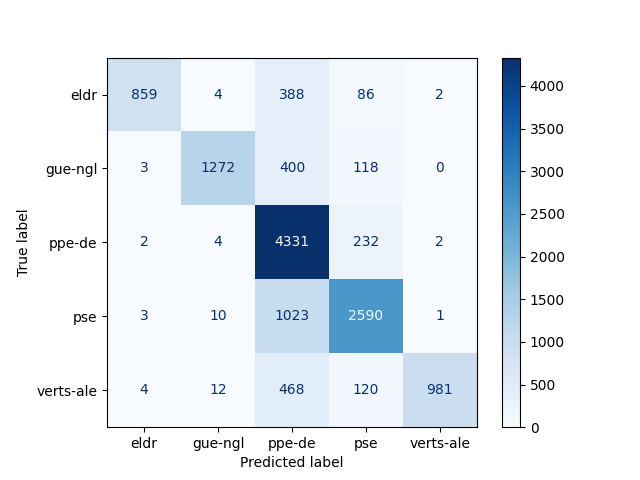
\includegraphics[width=0.5\textwidth]{matriceConfusionrandomforesten}
\caption{Matrice de confusion de randomForest en anglais}
\centering
\end{figure}

\begin{table}[h]
\centering
\begin{tabular}{lccc}
\hline
 & precision & recall & f-score\\
\hline
ELDR & 0.99 & 0.61 &  0.76\\
GUE-NGL&0.97  &0.71 & 0.82\\
PPE-DE & 0.64  &0.95  &0.76 \\ 
PSE &  0.83  &  0.69   &0.76 \\ 
Verts-ALE &  1.00   & 0.61 &  0.76\\
\hline
accuracy& & &    0.77 \\
macro avg &  0.89 & 0.72 &  0.77 \\
weighted avg &  0.82 &0.77 &0.77 \\
\hline
\end{tabular}
\caption{rapport de classification pour le modèle SGD Classifier en italien}
\label{tab:randomForestit}
\end{table}

\begin{figure}[h]
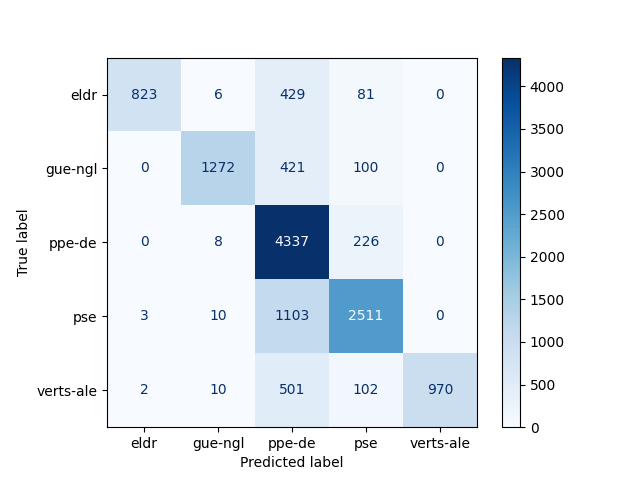
\includegraphics[width=0.5\textwidth]{matriceConfusionrandomForestit}
\caption{Matrice de confusion de randomForest en italien}
\centering
\end{figure}

\subparagraph{}
Les modèles d'apprentissage pre-transformers ne semblent donc pas capable de saisir la totalité de la tâche. On imagine obtenir de meilleurs résulats avec des modèles transformers de type BERT.


\end{document}
